\documentclass[12pt]{article}
\usepackage[utf8]{inputenc}
\usepackage{amsmath}                         % math
\usepackage[letterpaper, portrait, margin=1in]{geometry}
\usepackage{amsfonts}                        % math symbols (ex: R^n)
\usepackage{amssymb}

\usepackage{graphicx}                        % imagens
\usepackage{hyperref}                        % hyperlink
\usepackage[usenames, dvipsnames]{color}
\usepackage{algpseudocode}
\usepackage{listings}
\lstdefinestyle{term}
{
    backgroundcolor=\color{black},
    basicstyle=\footnotesize\color{white}\ttfamily
}

\algrenewcommand\Return{\State \algorithmicreturn{} } % removes returns in the same line for code 
\usepackage{indentfirst}
\usepackage{enumitem}
\setlist[description]{leftmargin=\parindent,labelindent=\parindent}

% colors
\definecolor{title_color}{RGB}{60, 100, 200}
\definecolor{text_color}{RGB}{0, 0, 0}
\definecolor{section_color}{RGB}{25, 100, 75}
\definecolor{basic_dir}{RGB}{0, 255, 170}
\definecolor{svb}{RGB}{0, 50, 150}

% titles
\usepackage{titlesec}
\titleformat*{\section}{\LARGE\bfseries}

%\usepackage{helvet}
\renewcommand{\familydefault}{\sfdefault}

\title{420 Project}
\author{Gustavo Estrela de Matos}
\bigskip
\date{\today}

\begin{document}
\begin{titlepage}
\begin{center}
    \begin{flushleft}
        \textcolor{title_color} {
            \fontsize{2cm}{1em}\selectfont {Breaking the RSA with Reversible Multiplier Circuits\\}
        }
    \end{flushleft}
  
    \begin{flushleft}{
        \textcolor{text_color} {
        \href{mailto:estrela.gustavo.matos@gmail.com}{Gustavo Estrela de Matos} 925003559\\}
    }
    \end{flushleft}
    \today
\end{center}
\end{titlepage}

\newpage
\section{The Problem}
RSA is an algorithm for data encryption used in many different security system and considered one of safest nowadays. This algorithm is based on the difficulty of the problem of factorizing the product of two large prime numbers, known as Integer Factorization Problem, which has no polynomial algorithm to solve (not considering that there are some polynomial algorithms for this problem in quantum computers).

\subsection{How to Break RSA Security}
The RSA algorithm has two different keys, a public and a private one. The private key is composed by two large prime numbers and the public key is composed by the product of these two primes, therefore, if we are able to factorize the public key we can get the private key,  which allows us to decrypt the message.

As mentioned before, the problem of factorizing integers is a hard problem and until today no one was able to give a polynomial algorithm to solve it. In this project we focus on creating a heuristic to find the prime factors that compose the public key of the RSA and crack the code.

The heuristic we are going to implement is based on the creation of a circuit that performs a reversible multiplier. This circuit is going to be composed of toffoli gates, which is a gate composed of control points and a controlled point. In a toffoli gate the open (closed) control point is satisfied if the input bit is 1 (0) and when all the control points are satisfied we toggle the controlled point. The circuit of a reversible multiplier is simply a set of toffoli gates.

\begin{figure}[h]
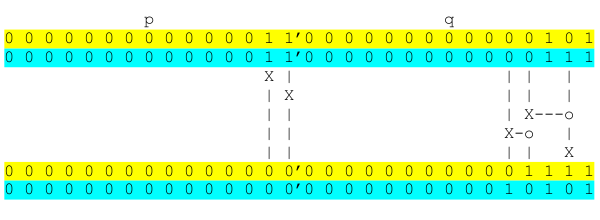
\includegraphics[scale=1.0]{MultiplierExample}
\caption{Example of a reversible Multiplier composed of toffoli gate. This multilpier is composed of five toffoli gates and it is capable of multiplying $3$ and $5$ (in yellow) and also $3$ and $7$ (in cyan). \emph{Figure available in http://courses.cse.tamu.edu/daugher/misc/PPP/homeworks/420-16spring-project.pdf}}
\end{figure}

\subsection{Goal of this Project}
In this project we intend to use search algorithms that we were exposed in class to solve the problem of finding the best multiplier possible, i.e the multiplier that correctly multiplies the greatest number of pairs of primes correctly. To do that we are going to use two search methods: genetic algorithms and local beam search. We are going to implement these two heuristics showing how we set up their parameters and also compare their efficiency.

\subsection{Restrictions and Limitations}
\label{restrictions}
It should be a know fact for the reader that the number of primes are infinite, therefore, as we explained before we do not intend to create a universal circuit capable of multiplying any pair of primes. The first limitation imposed in our algorithm is that toffoli gates and multilplier circuits only handle up to 30-bits number. Another limitation is that the input of a multiplier should be a 30-bits number $\overline{p}'\overline{q}$ where $\overline{p}$ and $\overline{q}$ are 15-bits representation of $p$ and $q$ respectively, and $p \leq q$, and this is what guarantee this circuit to be reversible (otherwise order changing would create a different solution).

In the development of this project we also had to restrict the number of primes that we were considering for multiplication, so then we would be able to see more effective results of both genetic algorithms and local beam search. Our limitation is that we are only considering the first fourty prime numbers, i.e primes between 2 and 173 (we can round up to 8 bit primes).

\section{Solving the Problem}
As mentioned before we implemented used two different approaches to solve this problem: genetic algorithms and local beam search. In this section we describe how we implemented the solution using these two different approaches and how we set up parameters for them based on experimentation.

\subsection{Solution Evaluation}
The first problem we faced in this project was to find a fast way to compute the fitness or the score of a solution. The first approach we used was to run the multiplier being tested to all possible combinations of 30-bits prime numbers. This approach showed to be too slow, which is not good because for both genetic algorithm and local beam search, the fitness function is called constantly.

To solve this problem we decided to add to our search method a parameter that stores the number of prime pairs (randomly chosen) that should be multiplied to calculate the fitness of a multiplier. This does not solve entirely the evaluation problem because now, since there are a lot of different pair of primes, it would be hard to distinguish a multiplier that works for one input from one that does not work for any input; that happens because the probability of choosing that one input is too small. Finally, we added a limit on the number of primes we consider for this problem, as we mentioned in the section \ref{restrictions}.

\subsubsection{Bit Entropy}
\label{bit-entropy}
Before explaining how we implemented both solutions present on this project we should understand the concept of entropy and how we can use it to guide our algorithms on the search for the best solution. In the context of this project we can define that the entropy of a bit is the inverse of the amount of information that this bit has, and by information we mean how certain are we that this bit needs to be toggled - or, complimentary, not toggled - from input to output. 

For instance, let's consider that the $i$-th bit has been correct for $90\%$ of the evaluations, then we can say that probably this bit will be correct for other pair of primes, and similarly, we can say that this bit will not be correct if it wasn't correct in the past evaluations. Knowing that, we can use this high informative bits to place our toffoli gates on bits that are normally incorrect and place the control points on bits that are normally correct.

\subsection{Genetic Algorithm}
The genetic algorithm approach consists of creating an initial set of multipliers, in this context called individuals, each one evaluated for some fitness function, and a sequence of iterations with crossovers and mutations. Each iteration generates a new generation of individuals that, in theory, should converge to a better fitting individual, which in this case is the individual that correctly multiplies the greates number of pairs of primes.

\subsubsection{Population Start}
Our first attempt to start the population 
\subsubsection{Crossover}
We tried two different approaches for crossing over two individuals $I_1$ and $I_2$, both of them considering the relative fitness:
\begin{itemize}
    \item{Random crossing: for every gate in $I_i$, add this gate with probability $RelativeFitness (I_i)$}
    \item{Column random crossing: for every gate controlling the $j-$th bit of $I_i$, add all these gates to the child with probability $RelativeFitness (I_i)$. If the sum of gates in the $j$-th column of both individuals is less than $5$, add all these gates to the child with probability $.5$.}
    After some tests we concluded that the second approach was more effective than the first one.
\end{itemize}

\subsubsection{Mutation}
The mutation happens right after the crossover with probability of $0.5$, and it exploits the Bit Entropy as we defined in section \ref{bit-entropy}. The mutation only adds new gates to the child multiplier, placing the gate on a bit that is frequently incorrect with up to $6$ (random) control points placed in frequently correct bits. We also tried totally random gates, but that haven't shown to be effective.

\subsubsection{Fitness Function}
The fitness function used in the genetic algorithm is simlpy the number of correct multiplications seen when evaluated the individual.

\subsection{Local Beam Search}
\subsubsection{Fitness Function}
\subsubsection{Choosing Next Step}


\section{Results}
\subsection{Sample Run}
\subsection{Analysis}


\section{Conclusion}
\subsection{Lessons Learnt}
\subsection{Future Research}
\end{document}
